%%%%%%%%%%%%%%%%%%%%%%%%%%%%%%%%%%%%%%%%%
% Short Sectioned Assignment
% LaTeX Template
% Version 1.0 (5/5/12)
%
% This template has been downloaded from:
% http://www.LaTeXTemplates.com
%
% Original author:
% Frits Wenneker (http://www.howtotex.com)
%
% License:
% CC BY-NC-SA 3.0 (http://creativecommons.org/licenses/by-nc-sa/3.0/)
%
%%%%%%%%%%%%%%%%%%%%%%%%%%%%%%%%%%%%%%%%%

%----------------------------------------------------------------------------------------
%	PACKAGES AND OTHER DOCUMENT CONFIGURATIONS
%----------------------------------------------------------------------------------------

\documentclass{article} % A4 paper and 11pt font size

\usepackage[T1]{fontenc} % Use 8-bit encoding that has 256 glyphs
\usepackage[english]{babel} % English language/hyphenation
\usepackage{amsmath,amsfonts,amsthm} % Math packages

\usepackage{graphicx}
\usepackage{pdfpages}
\usepackage{algorithm}
\usepackage[noend]{algpseudocode}
\usepackage{listings}
\usepackage{color}

\definecolor{dkgreen}{rgb}{0,0.6,0}
\definecolor{gray}{rgb}{0.5,0.5,0.5}
\definecolor{mauve}{rgb}{0.58,0,0.82}

\lstset{frame=tb,
  language=C,
  aboveskip=3mm,
  belowskip=3mm,
  showstringspaces=false,
  columns=flexible,
  basicstyle={\small\ttfamily},
  numbers=none,
  numberstyle=\tiny\color{gray},
  keywordstyle=\color{blue},
  commentstyle=\color{dkgreen},
  stringstyle=\color{mauve},
  breaklines=true,
  breakatwhitespace=true,
  tabsize=3
}

\makeatletter
\def\BState{\State\hskip-\ALG@thistlm}
\makeatother
%\usepackage{hyperref}

\usepackage{sectsty} % Allows customizing section commands
\allsectionsfont{\normalfont} % Make all sections centered, the default font and small caps
\usepackage{tikz}
\usetikzlibrary{arrows}

\newtheorem{definition}{Definition}

%\usepackage{titlesec}
%\titleformat*{\subsubsection}{\bfseries}

\usepackage[margin=1in]{geometry}
\usepackage{placeins}

\usepackage{fancyhdr} % Custom headers and footers
\pagestyle{fancyplain} % Makes all pages in the document conform to the custom headers and footers
\fancyhead{} % No page header - if you want one, create it in the same way as the footers below
\fancyfoot[L]{} % Empty left footer
\fancyfoot[C]{} % Empty center footer
\fancyfoot[R]{\thepage} % Page numbering for right footer
\renewcommand{\headrulewidth}{0pt} % Remove header underlines
\renewcommand{\footrulewidth}{0pt} % Remove footer underlines
\setlength{\headheight}{12pt} % Customize the height of the header
\setlength{\parskip}{1em}

\numberwithin{equation}{section} % Number equations within sections (i.e. 1.1, 1.2, 2.1, 2.2 instead of 1, 2, 3, 4)
\numberwithin{figure}{section} % Number figures within sections (i.e. 1.1, 1.2, 2.1, 2.2 instead of 1, 2, 3, 4)
\numberwithin{table}{section} % Number tables within sections (i.e. 1.1, 1.2, 2.1, 2.2 instead of 1, 2, 3, 4)

\setlength\parindent{0pt} % Removes all indentation from paragraphs - comment this line for an assignment with lots of text

%----------------------------------------------------------------------------------------
%	TITLE SECTION
%----------------------------------------------------------------------------------------

\newcommand{\horrule}[1]{\rule{\linewidth}{#1}} % Create horizontal rule command with 1 argument of height

\title{
\normalfont \normalsize
\textsc{Barcelona Graduate School of Economics} \\ [20pt] % Your university, school and/or department name(s)
\horrule{0.5pt} \\[0.1cm] % Thin top horizontal rule
\Large Efficient Estimation of Dynamic Conditional Correlation Models \\ % The assignment title
\horrule{0.5pt} \\[0.1cm] % Thick bottom horizontal rule
}

\author{Euan Dowers} % Your name

\date{\normalsize\today} % Today's date or a custom date

\begin{document}

\maketitle % Print the title

\pagebreak

\tableofcontents

\pagebreak

%----------------------------------------------------------------------------------------
% NEW SECTION
%----------------------------------------------------------------------------------------

\section{Introduction}

Estimating the correlation structure of a large number of financial assets is an important task for mean-variance optimisation, but is also an extremely difficult task, especially when the requirement is added that this correlation structure varies over time.

The aim of this paper is to efficiently estimate the Dynamic Conditional Correlation model in large dimensions (both in time and the number of assets included in the model), using two innovations. The first, due to Engle, Ledoit and Wolf \cite{engle ledoit and wolf}, is to use the linear shrinkage method of Ledoit and Wolf \cite{ledoit and wolf} to estimate the correlation targeting matrix of the DCC model, and the second, which is original to this paper, is to calculate the log-likelihood of the DCC model using a series of rank-one updates to the cholesky decomposition of the quasi-correlation matrix at each time period, thus avoiding having to refactor this matrix at every time period.

The structure of this report is as follows: Section \ref{section: dcc} will describe the Dynamic Conditional Correlation model, including the estimation problem; Section \ref{section: shrinkage} will describe the linear shrinkage estimation for covariance matrices of Ledoit and Wolf.

%----------------------------------------------------------------------------------------
% NEW SECTION
%----------------------------------------------------------------------------------------

\section{Dynamic Conditional Correlation Model} \label{section: dcc}

In order to describe the Dynamic Conditional Correlation Model, it is necessary to build up some notation.
\begin{enumerate}
  \item Let $r_{i,t}$ denote the return of asset $i$ at time $t$, and $r_t$ be the $N$-dimensional vector of all returns at time $t$.
  \item Let $\sigma_{i,t}^2 = V_{t-1}(r_{i,t} | \mathcal{F}_{t-1})$ be the conditional variance of asset $i$ at time $t$, given information up to time $t-1$.
  \item Let $D_t$ be a diagonal matrix such that $D_{i,i,t} = \sigma_{it}$.
  \item Let $H_t$ denote the conditional covariance matrix such that $H_{i,i,t} = \text{cov}_{t-1}(r_{i,t}, r_{j,t} | \mathcal{F}_{t-1})$.
  \item Let $\epsilon_{i,t} = \frac{r_{i,t}}{\sigma_{i,t}}$ be the standardised residual of asset $i$ at time $t$.
  \item Let $R_t$ be the conditional correlation matrix, whose i,j-th entry is given by the conditional correlation between asset $i$ and asset $j$ at time $t$.
  \item Let $\sigma_i^2$ be the unconditional variance of the series $r_i,t$
  \item Let $R$ be the unconditional correlation matrix of the system.
\end{enumerate}

%----------------------------------------------------------------------------------------

In the simpler \emph{Constant Conditional Correlation} model, the conditional correlations between pairs of assets are time-independent. In particular
\begin{equation}
  H_{i,j,t} = \rho_{i,j}\sqrt{H_{ii,t}H_{jj,t}}
\end{equation}
and thus
\begin{equation}
H_t = D_tRD_t, \ D_t = \text{diag}(H_t)^{1/2}
\end{equation}

The DCC model is a natural generalisation of this model, in that it allows the conditional correlations to vary over time. The DCC model first expresses the volatility structure of assets independently, and then the correlations between returns in another. If we have two series of returns $r_i, r_j$, the conditional correlation between them is given by
\begin{equation}
  \rho_{i,j,t} = \frac{E_{t-1}((r_{i,t} - E_{t-1}(r_{i,t}))(r_{j,t} - E_{t-1}(r_{j,t})))}
                      {\sqrt{V_{t-1}(r_{i,t})V_{t-1}(y_{j,t})}},
\end{equation}
and therefore
\begin{equation}
\rho_{i,j,t} =  \frac{H_{i,j,t}}{\sqrt{H_{i,i,t}H_{j,j,t}}}.
\end{equation}
Therefore, the conditional correlation matrix and conditional variance matrix are given by
\begin{equation}
  R_t = D_t^{-1} H_t D_t ^{-1} \ \  D_t ^2 = diag[H_t].
\end{equation}
It therefore follows that the conditional correlation matrix is given by the conditional covariance matrix of the standardised residuals
\begin{equation}
R_t = V_{t-1} (D_t^{-1}y_t) = V_{t-1}(\epsilon_t).
\end{equation}
Therefore, we only need to look at the standardised residuals of each series. The first step in fitting any DCC model is therefore to extract the standardised residuals, a problem that has been given much attention in the literature. For the purpose of this paper, I use only a GARCH(1,1) process, but software to estimate other volatility models (TARCH, APARCH, EGARCH) exists and can be used as is necessary.

There are several common specifications for the dynamics of the conditional correlation matrix. In the mean-reverting DCC model, the dynamics of the quasi-correlation matrix $Q_t$ are governed by the process
\begin{equation} \label{correlation targeting}
  Q_t = \Omega + \alpha \epsilon_{t-1}\epsilon_{t-1}' + \beta Q_{t-1}.
\end{equation}
We can see that for each entry of the matrix $Q_t$, the dynamics are given by
\begin{equation}
Q_{i,j,t} = \omega_{i,j} + \alpha \epsilon_{i,t-1}\epsilon_{j,t-1} + \beta Q_{t-1},
\end{equation}
from which the comparison with the GARCH(1,1) model is clear. Clearly, the intercept matrix $\Omega$ introduces $N(N-1)/2$ free parameters into the model, but in the \emph{correlation targeting} version of this model, the intercept matrix $\Omega$ is given
\begin{equation}\label{eq: correlation targeting}
  \Omega = (1 - \alpha - \beta)\bar{R}
\end{equation}

Then, to convert the matrix $Q_t$ into a correlation matrix we just divide the $i,j$-th entry by $\sqrt{Q_{i,i,t}Q_{j,j,t}}$, ie
\begin{equation}
  R_t = \text{diag}\{Q_t\}^{-\frac{1}{2}} Q_t \text{diag}\{Q_t\}^{-\frac{1}{2}}
\end{equation}
This model is the \textit{mean reverting} DCC model because we can see that over time as shocks to the correlation structure of the system decay, the system will tend towards its mean.

We will discuss in Section \ref{section: dcc estimation} how the DCC model is estimated in practice, and the difficulty of doing so when the number of assets considered, $N$, is large.

%----------------------------------------------------------------------------------------
% NEW SECTION
%----------------------------------------------------------------------------------------

\section{Shrinkage Estimation for Large Unconditional Correlation Matrices}\label{section: shrinkage}

As seen in Equation ref{eq: correlation targeting}, a key part of fitting the DCC model is estimating the covariance matrix of the standardised residuals. We know from the cross-sectional literature that using the sample covariance matrix, in Equation \ref{eq: sample_covariance}, works poorly in large dimensions, since for large $N$, with $N \approx T$, the sample covariance matrix contains a lot of estimation error, since the correlation matrix has to estimate $\frac{N(N-1)}{2}$ parameters with $T$ data points, so is prone to overfitting and provides a good fit in-sample but generalises poorly.

 The \textit{shrinkage} estimator of the covariance matrix aims to solve this problem of estimating the covariance matrix in high dimensions, essentially by first showing that the largest eigenvalues of the sample covariance matrix are larger than the true values, and the smallest eigenvalues are smaller than their true values. Therefore, if we \textit{shrink} the sample eigenvalues towards their true value we should get a better estimate of the sample covariance matrix. Let $\Sigma$ denote our true covariance matrix and $\hat{\Sigma}$ denote our sample covariance matrix. Further, let $\hat{\lambda}_i$ denote the $i$-th largest eigenvalue of $\hat{\Sigma}$.

\begin{equation} \label{eq: sample_covariance}
\hat{\Sigma} = \frac{1}{T} \sum \epsilon_t \epsilon_t'
\end{equation}

The \textit{linear shrinkage} estimator of the covariance matrix, given by Ledoit and Wolf, aims to find the optimal linear combination
\begin{equation}
\Sigma* = \rho_1 I + \rho_2 \hat{\Sigma}
\end{equation}
such that the expected loss $\mathbb{E}||\Sigma^* - \Sigma||^2$ is minimal, where $||A||$ is the Frobenius norm of $A$, where for $A \in \mathbb{R}^{m \times n}$
\begin{equation}
||A|| = \sqrt{\text{trace}(AA')}.
\end{equation}
Ledoit and Wolf find an optimal, nonrandom solution for $\rho_1, \rho_2$, but it requires prior knowledge about the true covariance matrix $\Sigma$. In particular, we need to be able to calculate the following values

\begin{align}
\mu &= \langle \Sigma , I \rangle \nonumber \\
\alpha^2 &= || \Sigma - \mu I ||^2 \nonumber \\
\delta^2 &= \mathbb{E}||\hat{\Sigma} - \mu I ||^2.
\end{align}

Given these four scalar values, Ledoit and Wolf give a nonrandom optimal linear shrinkage estimator. Consider the problem we are trying to solve:

\begin{align}
\nonumber
\min\limits_{\rho_1, \rho_2} \mathbb{E} \left[ || \Sigma^* - \Sigma ||^2 \right]\\
s.t  \ \Sigma ^* = \rho_1 I + \rho_2 \hat{\Sigma}.
\end{align}
Ledoit and Wolf show that this problem is solved by
\begin{equation}
\Sigma ^* = \frac{\beta^2}{\delta^2} \mu I + \left(1 - \frac{\beta^2}{\delta^2}\right) \hat{\Sigma}
\end{equation}

Obviously, however, we do not know the true covariance matrix, so we cannot directly compute these values and the optimal shrinkage intensity, $rho$. However, Ledoit and Wolf show the following constants can be combined to give a consistent estimator of the optimal shrinkage intensity.

\begin{align}
\nonumber
m &= \langle \hat{\Sigma}, I \rangle \\
\nonumber
d^2 &= ||\hat{\Sigma} - mI||^2_n \\
\nonumber
\bar{b}^2 &= \frac{1}{^2} \sum\limits_{k=1}^{T} ||\epsilon_t \epsilon_t' - \hat{\Sigma}||^2 \\
b^2 &= \min(\bar{b}^2, d^2)
\end{align}

A consistent estimator for the optimal shrinking intensity $\hat{\rho}$ is then given by
\begin{equation}\label{rho hat}
\hat{\rho} = \frac{b^2}{d^2}
\end{equation}
and then, our linear shrinkage estimate of the covariance matrix is
\begin{equation}
\bar{C} = \sum\limits_{i = 1}^{N}\left[ \hat{\rho}\bar{\lambda} + (1 - \hat{\rho}) \hat{\lambda}_i \right] u_i u_i'
\end{equation}


By a property of the Frobenius norm, the value $\mu$ is related to the eigenvalues of $\Sigma$, $\hat{\lambda}_i$ by the equation
\begin{equation}
\mu = \frac{1}{N} \sum\limits_{i=1}^{N} \lambda_i = \mathbb{E} \left[ \frac{1}{N} \sum\limits_{i=1}^{N} \hat{\lambda}_i \right]
\end{equation}

Ledoit and Wolf also show \cite{non-linear shrinkage} that using a non-linear version of shrinkage estimation works better, but employing this technique is beyond the scope of this paper, and is an opportunity for further research. The main difference being that in nonlinear shrinkage the shrinkage parameter $\rho$ is determined for each eigenvector individually rather than being forced to be the same for each eigenvector.

%----------------------------------------------------------------------------------------
% NEW SECTION
%----------------------------------------------------------------------------------------

\section{DCC Model Estimation}\label{section: dcc estimation}

In Section

The problem of estimating the DCC model can be formulated as a maximum likelihood problem. In the DCC model where the conditional distribution of $r_t$

\begin{equation}\label{eq: loglik}
l = - \frac{1}{2} \sum\limits_{t=1}^T n \log(2\pi) + 2 \log |D_t| + y_t' D_t^2y_t - \epsilon_t' \epsilon_t + \log |R_t| + \epsilon_t'R_t^{-1}\epsilon_t
\end{equation}

This log-likelihood can be split into two parts, the first part contains only the variane parameters from the GARCH specification in Equation \ref{eq: garch}, and the second contains only the DCC parameters, $\alpha$ and $\beta$. This log-likelihood can therefore be maximised in two stages, the first maximising with respect to the variance parameters $\omega_i, \alpha_i, \beta_i$, and the second stage maximising with respect to $\alpha, \beta$. The first stage is done by fitting a univariate GARCH(1,1) model to each asset independently.

To model the quantities $d_{i,t}$, and from this extract the standardised residuals $\epsilon_t$ we apply the univariate GARCH(1,1) model to each asset serparately to obtain the dynamics of its conditional variance.
\begin{equation}\label{eq: garch}
  H_{i,i,t} = \omega_i + \alpha_i r_{t-1}^2 + \beta_i H_{i,i,t-1}.
\end{equation}
 Then, the standardised residuals $\epsilon _{i,t}$ are given by
 \begin{equation}
\epsilon_{i,t} = \frac{r_{i,t}}{d_{i,t}}
 \end{equation}

For the second stage, after fitting our univariate, independent GARCH(1,1) models, we extract the standardised residuals $\epsilon_{i,t}$ and use these to calculate the second part of the log-likelihood function

\begin{equation}\label{eq: L2}
l_2 = -\frac{1}{2}\sum\limits_{t=1}^{T} \log |R_t| + \epsilon_t'R_t^{-1}\epsilon_t.
\end{equation}

To clarify how this relates to the specification of the mean-reverting DCC model in terms of $\alpha$ and $\beta$, let us remind ourselves of the dynamics of the quasi-correlation matrix $Q_t$, and how $Q_t$ relates to the conditional correlation matrix $R_t$.
\begin{align}
Q_t
&= \Omega + \alpha \epsilon_{t-1}\epsilon_{t-1}' + \beta Q_{t-1}, \\
\text{and } R_t
&= \text{diag}\{Q_t\}^{-\frac{1}{2}} Q_t \text{diag}\{Q_t\}^{-\frac{1}{2}}.
\end{align}

Therefore, in order to calculate the log-likelihood of our observed data, we need to, at every time interval $t$, invert the matrix $R_t$. Therefore, if $T$ or $N$ is large, directly estimating the log-likelihood in a naive way (by calculating the inverse of the matrix $R_t$ for each $t \in \{1, \ldots , T\}$) becomes computationally infeasible.

\subsection{Cholesky Decomposition}

The first thing to note is that we do not ever calculat the inverse of the matrix $R_t$. Rather we use the \textit{Cholesky decomposition}, where, for a positive definite matrix $A$, $A = LL'$, where $L$ is a lower triangular matrix.
\begin{equation}
  L=
    \begin{bmatrix}
      L_{11} & 0      & 0       \\
      L_{21} & L_{22} & 0       \\
      L_{31} & L_{32} & L_{33}  \\
    \end{bmatrix}.
\end{equation}
This allows us to solve the system of linear equations $Ax = b$ (and thus $x = A^{-1}b$) using forward and back-substitution, without having to calculate $A^{-1}$. In particular, we want to, at each time interval $t$, calculate the quantity $R_t^{-1}\epsilon_t$. So, given the Cholesky decomposition of the matrix $R_t$, $\tilde{L}_t$ we can compute $x_t = R_t^{-1}\epsilon$ and therefore $ = \epsilon_t'x_t = \epsilon_t'R_t^{-1}\epsilon_t$, the second part of $l_2$. Therefore, if we can come up with a way of updating the cholesky decomposition of $R_t$ at each time interval $t$, without having to refactor, then we can improve on the computational complexity of the log-likelihood calculation.

\subsection{Updating the Cholesky Decomposition}

Fortunately, there are algorithms for updating the cholesky decomposition of a matrix $A$ when $A$ is modified by
\begin{equation}
\tilde{A} = A + x'x
\end{equation}
where $x$ is a vector of length $N$. Such an update is called a rank one update, and the algorithm implemented for finding the Cholesky decomposition of $\tilde{A}$ is given by Algorithm \ref{rank one update}

\begin{algorithm}
\caption{Rank One Update to Cholesky decomposition}\label{rank one update}
\begin{algorithmic}[1]
\Procedure{RankOneUp}{}
\For {$i \in 1:N$}
\State $r \gets \sqrt{L_{ii}^2 + x_i^2}$
\State $c \gets r / L_{ii}$
\State $s \gets x_i/L_{ii}$
\For {$j \in i+1:N$}
\State $L_{ji} \gets \frac{L_{ji} + sx_{j}}{c}$
\State $x_j \gets c x_j - sL_{ji}$
\EndFor
\EndFor
\EndProcedure
\end{algorithmic}
\end{algorithm}

Noting that if we take $x$ to be $\sqrt{\frac{\alpha}{\beta}}\epsilon_t$, this gives us an algorithm for finding the Cholesky decomposition of $Q_{t-1} + \frac{\alpha }{\beta}\epsilon_t \epsilon_t'$. Now note that if we multiply the resulting decomposition $\tilde{L}$ by $\sqrt{\beta}$ we get the Cholesky decomposition of $\alpha \epsilon_t' \epsilon_t + \beta Q_{t-1}$. Therefore, this algorithm has given us an efficient way to update the Cholesky decomposition of the quasi-correlation matrix $Q_t$. However, the problem occurs when we add the full rank correlation target matrix $\Omega$. There is no way of updating the Cholesky decomposition upon adding a full-rank matrix that is any more efficient than refactoring the matrix $Q_t$ at every time interval $t$.

The innovation of this paper is to approximate each update by using the linear shrinkage estimator for the covariance matrix. In particular, rather than adding the full $\Omega$ matrix at each time step, we add the $n$ largest eigenvalues. This allows us to estimate the true log-likelihood of some given DCC parameters, $\hat{\alpha}$ and  $\hat{\beta}$, a process summarised in Algorithm \ref{alg: loglik}, where the inputs are a matrix of returns, where $r_{it}$ is the return of asset $i$ at time $t$, and DCC parameter estimates $\alpha$, $\beta$

\begin{algorithm}[h]
\caption{Estimating log-likelihood}\label{alg: loglik}
\begin{algorithmic}[1]
\Procedure{LogLik}{}
\For {$i \in 1:N$}
\State Fit GARCH(1,1) model to $r_i$
\State $\epsilon_{it} \gets r_{it} / \hat{\sigma}_{it}$
\EndFor
\State $\hat{\Sigma} \gets \frac{1}{T}\sum\limits_{i=1}^T \epsilon_t \epsilon_t'$
\State Calculate eigenvalues, eigenvectors of $\hat{\Sigma}$
\State $\hat{\lambda}_i \gets$ i-th largest eigenvalue; $u_i \gets$ corresponding eigenvector
\State $\bar{\lambda} \gets \sum\limits_{i = 1}^N \hat{\lambda}_i$
\State Calculate $\hat{\rho}$ as in Equation \ref{rho hat}
\For {$i \in 1:N$}
\State $\lambda_i \gets \hat{\rho}\bar{\lambda} + (1 - \hat{\rho})\hat{\lambda}_i$
\EndFor
\State $\bar{C} \gets \frac{1}{T} \sum\limits_{i = 1}^{T} \lambda_i u_i u_i'$
\State $Q_1 \gets \bar{C}$
\State $L \gets \text{chol}(Q_1)$
\State $l \gets 0$
\For {$t \in 2:T$}
\State $Q_{t} \gets (1 - \alpha - \beta) \sum\limits_{i = 1}^n \lambda_i u_i u_i' + \alpha \epsilon_t \epsilon_t' + \beta Q_{t-1}$
\State $L$ updated by Algorithm \ref{rank one update}
\State $l += \log{|R_t|} + \epsilon_t'R_t^{-1}\epsilon_t$ using $L$
\EndFor
\State \textbf{return} $l$
\EndProcedure
\end{algorithmic}
\end{algorithm}

If one were to update the matrix $Q_t$ at each step, the algorithm would require $N^3/3$ FLOPs at each iteration to perform the Cholesky decomposition, and then a further $N^2$

%----------------------------------------------------------------------------------------
% NEW SECTION
%----------------------------------------------------------------------------------------

\section{Monte Carlo Simulation}

\subsection{Setup of Simulations}

To evaluate our method for approximating the log-likelihood of the DCC model, we use Monte Carlo simulation. In particular, we take as unconditional correlation matrix the Toeplitz matrix where the entries of the first row are given by the sequence $(1, \frac{n-1}{n}, \ldots, \frac{1}{n})$ eg
\begin{equation}
  T=
    \begin{bmatrix}
      1 & \frac{2}{3}     &  \frac{1}{3}       \\
      \frac{1}{3} & 1 &  \frac{2}{3}        \\
       \frac{2}{3}  & \frac{1}{3} & 1  \\
    \end{bmatrix}.
\end{equation}
We then simulate the DCC model, where the volatilities of each stock are governed by a GARCH(1,1) model with the parameterisation
\begin{equation}
\sigma_{it} = 0.01 + 0.05 r_{t-1}^2 + 0.9\sigma_{i(t-1)},
\end{equation}
and the DCC parameters are $\alpha = 0.05$ and $\beta = 0.9$, as in Pakel et al \cite{pakel et al} and Engle et al \cite{engle et al}. At each Monte Carlo simulation, we simulate a DCC model with the above dynamics, and then we look at the performance of our estimation method (using the estimated bias of the parameter estimates). We do this for $N \in \{ 5,10,50,100,200\}$ and for each of these, we choose a number of candidate values for $n$, ranging from $1$ to $N$.

\subsection{Results}

Here we report the results from the Monte Carlo Simulations. As can be seen in Figures \ref{bias_alpha} and \ref{bias_beta}, increasing the number of rank one updates, $n$, to $N$ gives the least biased estimates of $\alpha$ and $\beta$, with this bias being around 10$\times$ higher for the $n$ less than $N$. An interesting finding is that the bias of $\alpha$ increases as more updates are made. This is counterintuitive since as you add more eigenvectors you obtain a more accurate approximation of $\Omega$, and so the estimated DCC parameters should be less biased. However, we see that in general, either using only a single rank-one update with the largest eigenvector or using $N$ rank-one updates with all eigenvectors gives the least biased results.

The fact that in most Monte Carlo simulations the estimates $\hat{\alpha}$ and $\hat{\beta}$ are such that $\hat{\alpha} + \hat{\beta} \approx 1$ indicates that the impact of using only a few updates ($n < N$) rather than full updates, which in effect changes the correlation targeting matrix to
\begin{equation} \label{partial updates}
\Omega \equiv (1 - \alpha - \beta)\sum\limits_{i=1}^{n} \left( \hat{\rho}\bar{\lambda} + (1- \hat{\rho})\hat{\lambda_i} \right) u_i u_i'
\end{equation}
changes the correlation targeting matrix sufficiently that in the model it is so far from the true correlation targeting matrix that the optimal log-likelihood is to ignore it completely, biasing $\hat{\alpha}$ and $\hat{\beta}$ so $\hat{\alpha} + \alpha{\beta} \approx 1$. In the model, $\Omega$ has $N(N-1)/2$ free parameters, but in practice we just replace it with $(1 - \alpha - \beta)\bar{C}$, so in effect what using a small number of rank 1 eigenvector updates does is forces our choice of $\Omega$ to be a suboptimal one.

A potential solution to this would be if we could add a diagonal matrix $D$ to the update relation in Equation \ref{partial updates}, so the correlation target would be of the form
\begin{equation}
\Omega \equiv (1 - \alpha - \beta)\left[\sum\limits_{i=1}^{n} \left( \hat{\rho}\bar{\lambda} + (1- \hat{\rho})\hat{\lambda}_i \right) u_i u_i' + D\right].
\end{equation}
This would allow the correlation target to be diagonally dominant, with each diagonal element $\omega_{ii} \approx 1 - \alpha - \beta$. This would allow the correlation target to more accurately represent the true correlation targeting matrix, and should decrease the bias in our estimates. However, no such efficient scheme exists to update a Cholesky decomposition upon addition of a diagonal matrix, and so

\begin{figure}[h] \label{bias_alpha}
\begin{center}
\begin{tabular}{ |c|c|c|c|c| }
 \hline
 N/n & 5 & 10 & 50 & 100  \\
 \hline
 1 & 0.031 & 0.027 & 0.024 & -0.014  \\
 \hline
 5 & -0.012 & -0.035 & -0.028 & -0.032  \\
 \hline
 10 & - & 0.001 & -0.049 & 0.041  \\
 \hline
 50 & - & - & -0.003 & -0.009  \\
 \hline
 100 & - & - & - & 0  \\
 \hline
\end{tabular}
\end{center}
\caption{Bias of $\hat{\alpha}$ across simulations}
\end{figure}

\begin{figure}[h] \label{bias_alpha}
\begin{center}
\begin{tabular}{ |c|c|c|c|c|c| }
 \hline
 N/n & 5 & 10 & 50 & 100 & 200 \\
 \hline
 1 & -0.009 & -0.001 & -0.004 & 0.035 & 0\\
 \hline
 5 & -0.018 & 0.055 & 0.048 & 00.053 &  0\\
 \hline
 10 & - & -0.006 & 0.068 & 0.061 & 0 \\
 \hline
 50 & - & - & 0.006 & 0.028  & 0\\
 \hline
 100 & - & - & - & -  & 0\\
 \hline
\end{tabular}
\caption{Bias of $\hat{\beta}$ across simulations}
\end{center}
\end{figure}

\begin{figure}[h]
\begin{center}
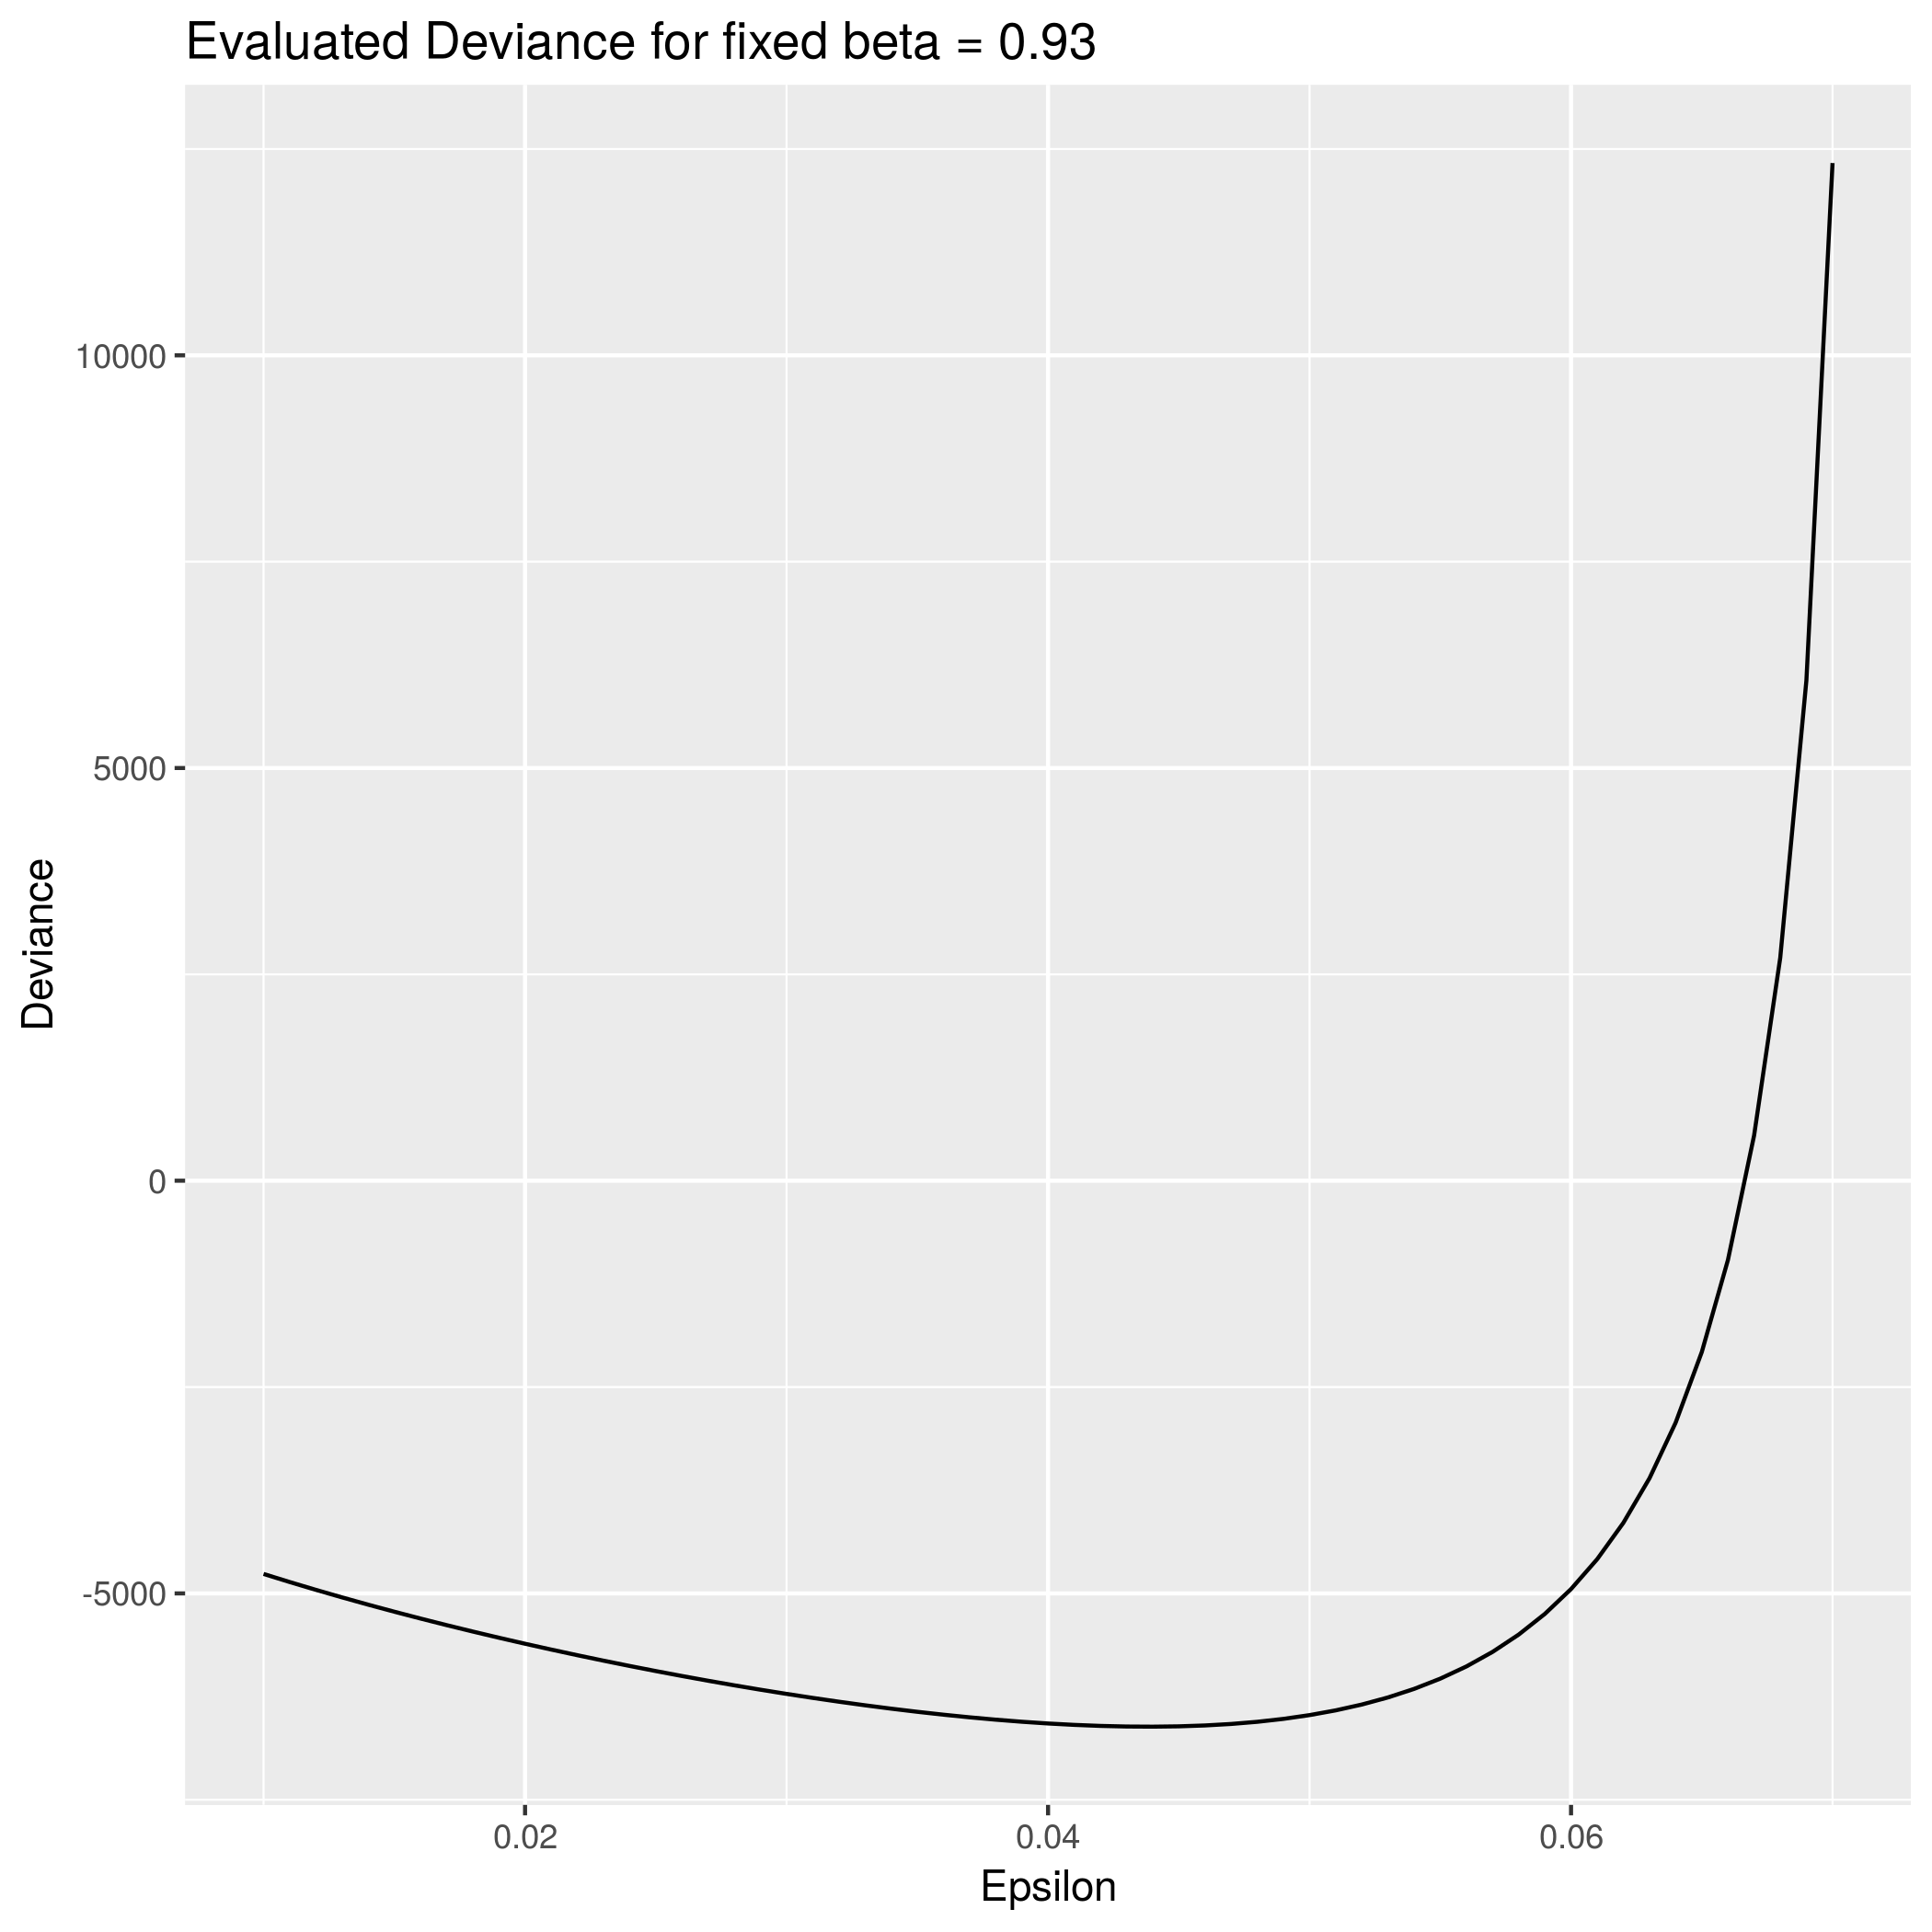
\includegraphics[scale = 0.5]{loglik1.png}
\caption{Estimated deviance for N = 20, n = 20}
\end{center}
\end{figure}

\begin{figure}[h]
\begin{center}
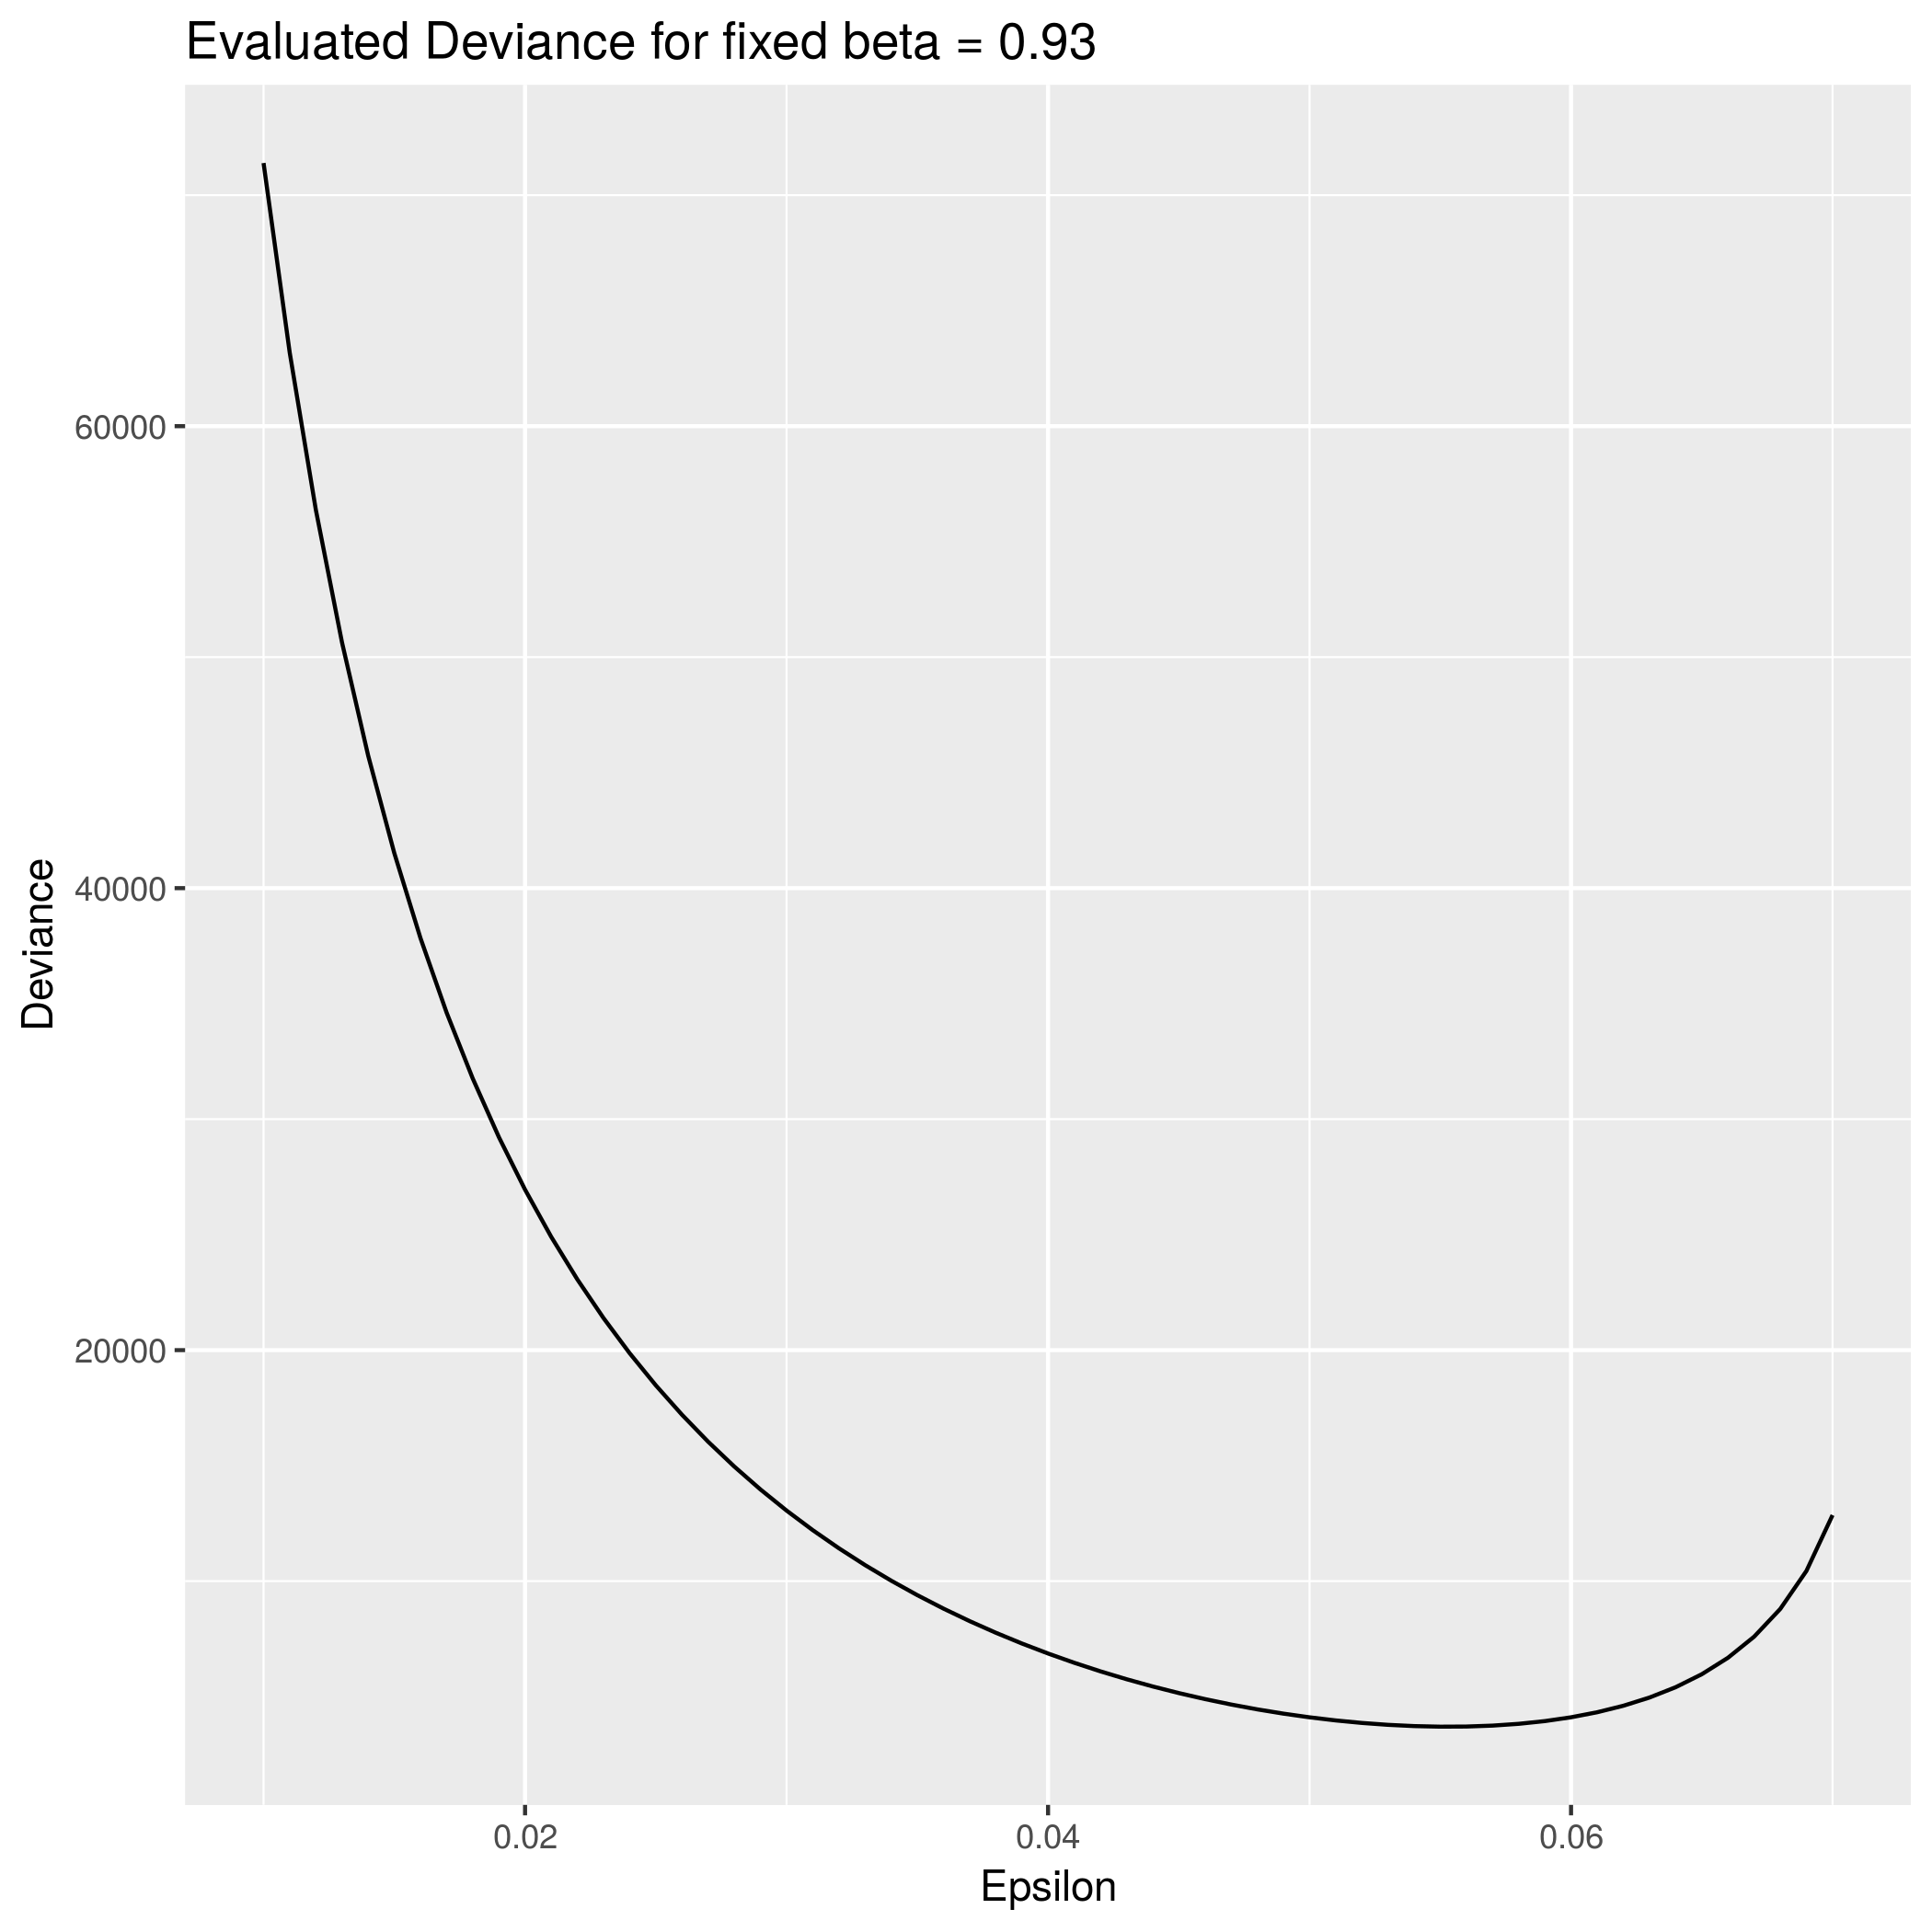
\includegraphics[scale = 0.5]{loglik2.png}
\caption{Estimated deviance for N = 20, n = 10}
\end{center}
\end{figure}

\begin{figure}[h]
\begin{center}
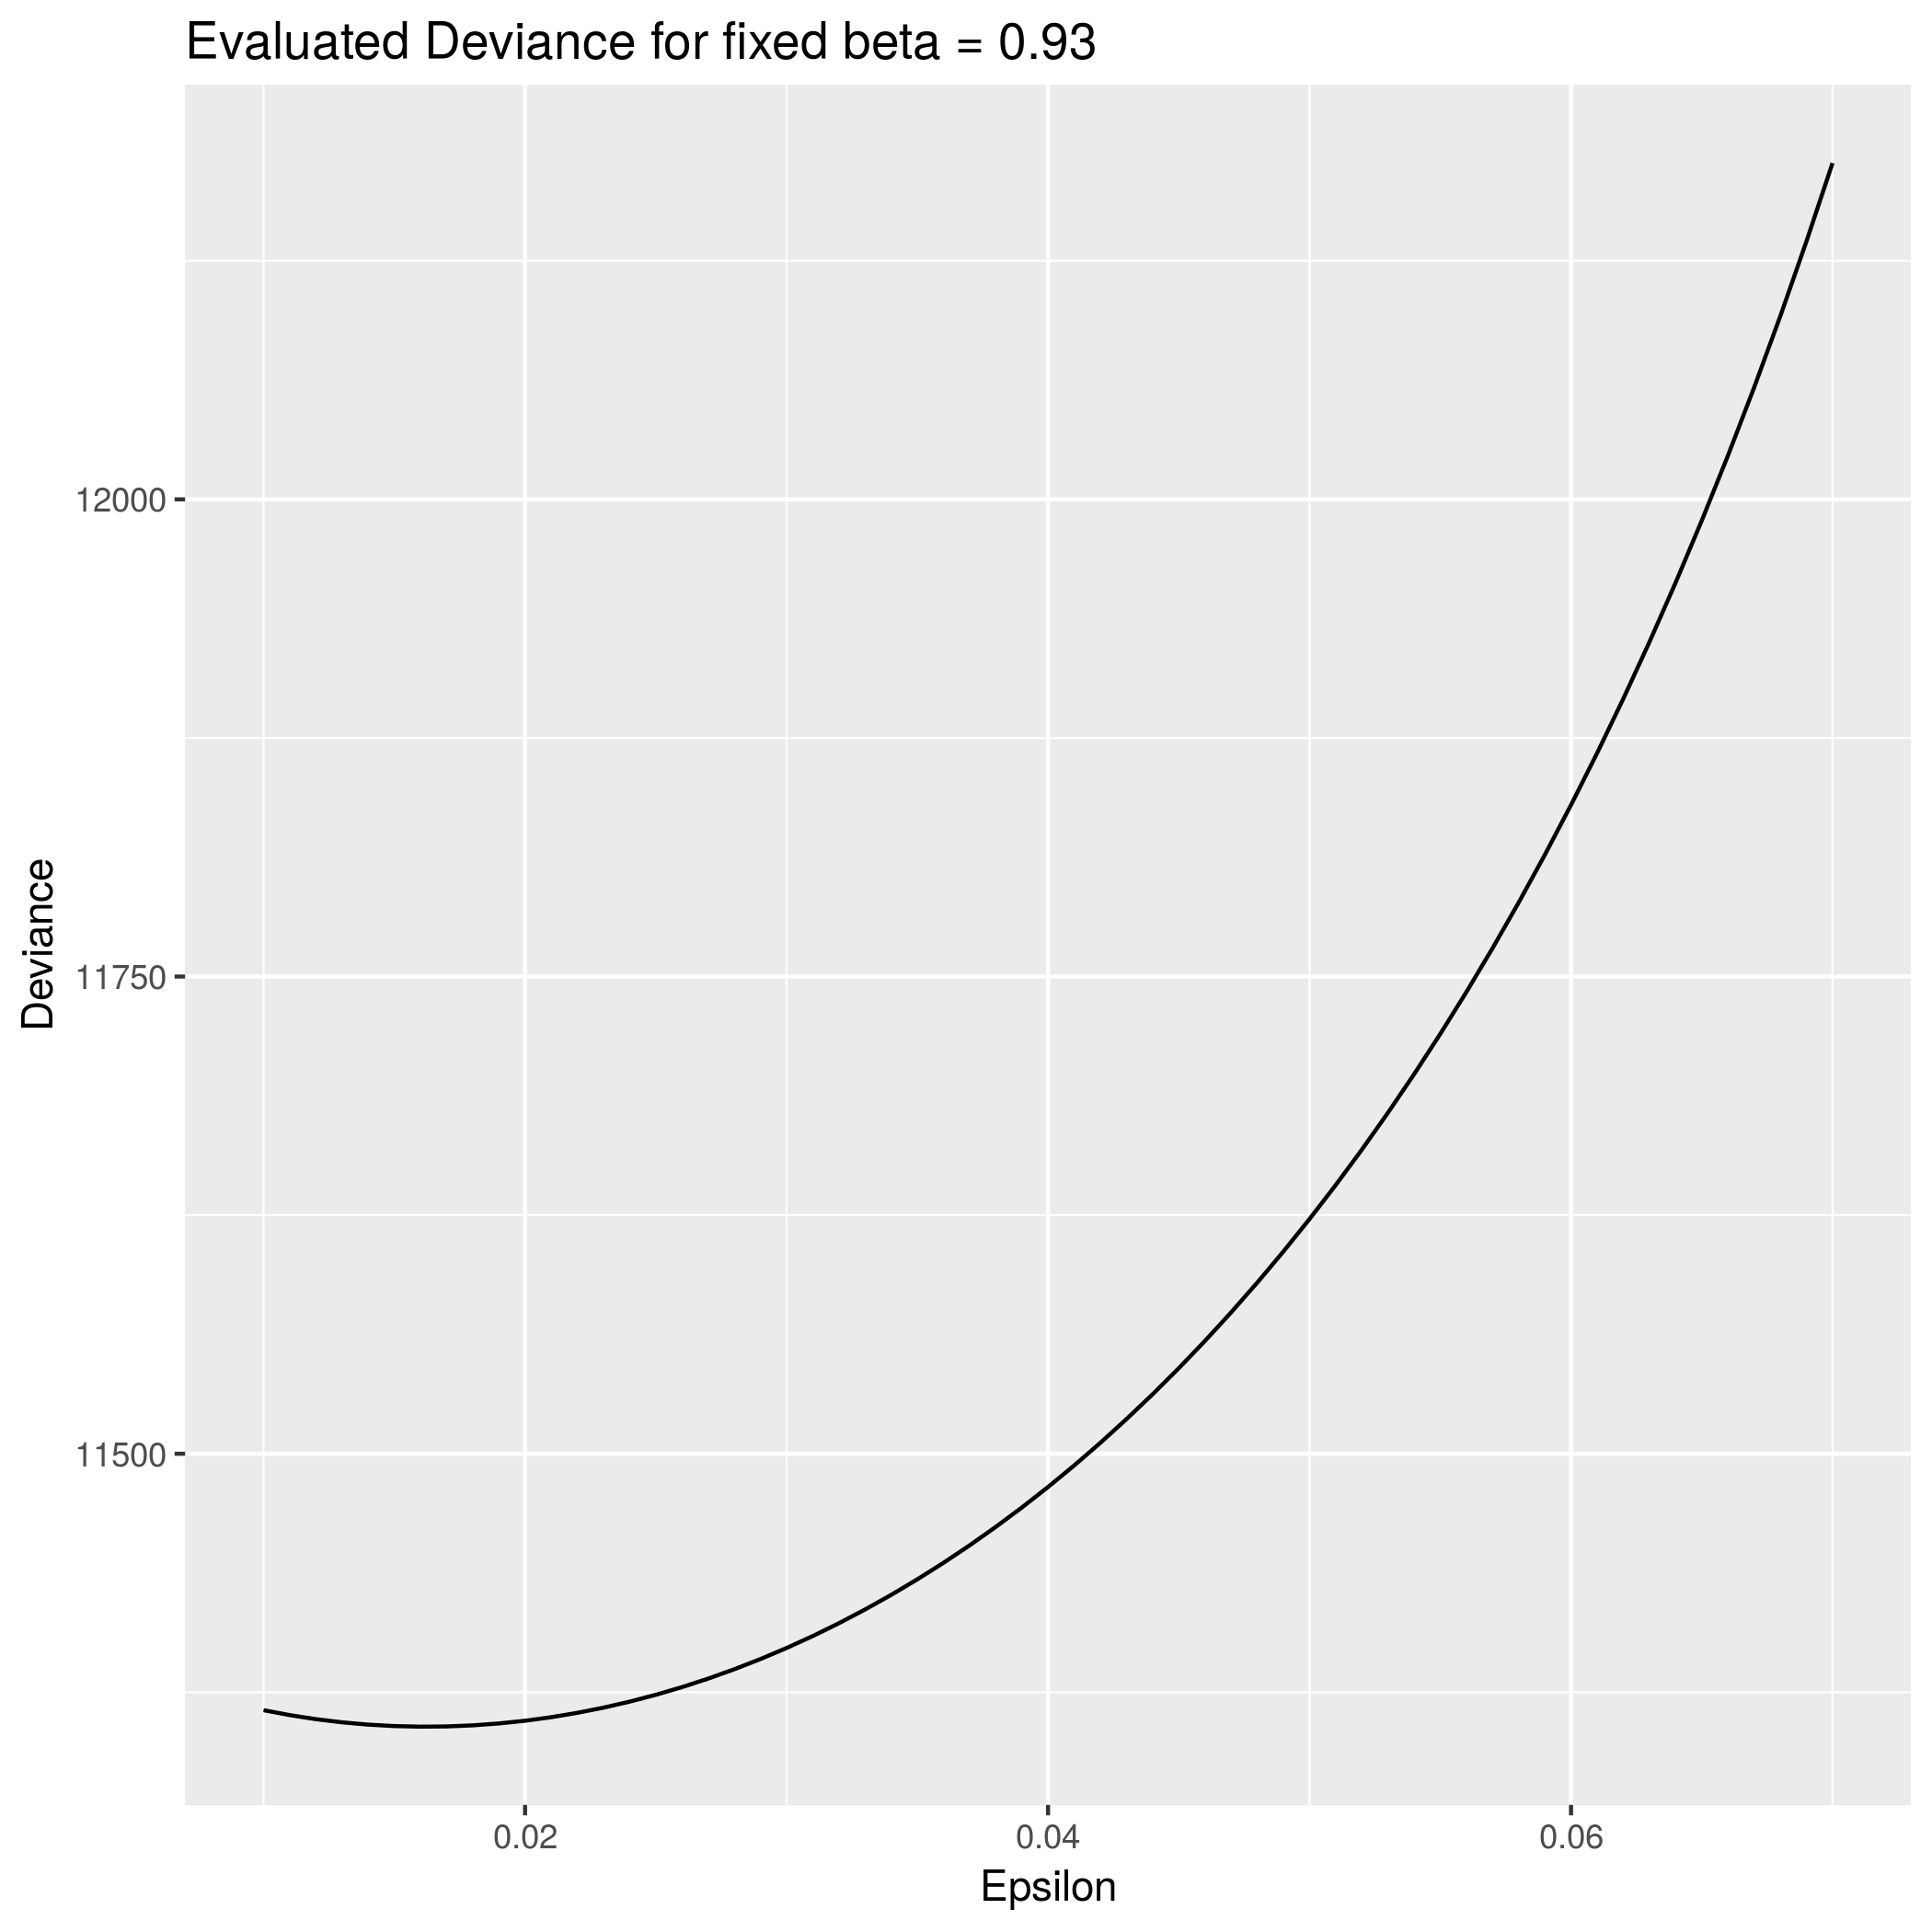
\includegraphics[scale = 0.5]{loglik3.png}
\caption{Estimated deviance for N = 20, n = 1}
\end{center}
\end{figure}

\FloatBarrier

%----------------------------------------------------------------------------------------
% NEW SECTION
%----------------------------------------------------------------------------------------

\section{Conclusion}

This thesis has proposed a method for efficiently estimating the parameters of a DCC model, using the linear shrinkage estimator of the covariance matrix as our correlation targeting matrix. The linear shrinkage estimator for the covariance matrix was used because it has been shown in the cross-sectional, static literature that this estimator is more robust in large dimensions, where the concentration ration $\frac{N}{T}$ is large. This was used to represent the

\pagebreak

\begin{thebibliography}{9}
\bibitem{engle2002}
Engle, R.
\textit{Dynamic Conditional Correlation - a simple class of multivariate models}.
Journal of Business and Economic Statistics, 2002.

\bibitem{bollerslev90}
Bollerslev, D
\textit{Dynamic Conditional Correlation - a simple class of multivariate models}.
Journal of Business and Economic Statistics, 1990.

\bibitem{anticipating correlations}
Engle, R.
\textit{Anticipating Correlations: a new paradigm for risk management}
\end{thebibliography}

\end{document}
